\documentclass[a4paper,11pt]{article}
\usepackage[utf8]{inputenc}
\usepackage[frenchb]{babel}
\usepackage{amssymb}
\usepackage{amsmath}
\usepackage{amsthm}
\usepackage{mathrsfs}
\usepackage{array}
\usepackage{graphicx}
\usepackage[usenames,dvipsnames]{color}
\usepackage{listings}
\usepackage{arydshln}
\usepackage{slashbox}
\usepackage{subfigure}
\usepackage{pdflscape}
\usepackage{multirow}
%\usepackage{cancel}
%\usepackage[bookmarks = false]{hyperref}
\usepackage{enumitem}
\usepackage[left=1.75cm, right=1.75cm, top=2cm, bottom=2cm]{geometry}

\newcommand{\ttsee}[1]{Voir \texttt{#1}\paragraph{}}
\newcommand{\ttseek}[1]{Voir package \texttt{#1}\paragraph{}}


% Initialisation de listings
%\definecolor{mymauve}{rgb}{0.63,0.13,0.94}
%\definecolor{mygreen}{rgb}{0.13,0.55,0.13}
%\definecolor{mybeige}{rgb}{0.99,0.99,0.86}
\definecolor{bcg}{rgb}{0.95,0.95,0.95}
\definecolor{light-gray}{gray}{0.50}
\lstset{
	backgroundcolor=\color{bcg},   % choose the background color; you must add \usepackage{color} or \usepackage{xcolor}
    columns=flexible,
	%numbers = left,				    % placement de la numérotation des lignes
	numberstyle = \small,        	% taille du numéro de ligne
	stepnumber = 1,              	% ???
	numbersep = 10pt,            	% taille de l'espace de séparation entre numéro de ligne et code
	showspaces = false,          	% montrer les espaces
	showstringspaces=false,         % enlever les espaces str
	showtabs = false,            	% montrer les tabulations
	tab = rightarrowfill,        	% ???
	tabsize=2,						% tabulation size
	language = Java,             	% langage utilisé
	basicstyle = \footnotesize\tt,	% ???
	captionpos = b,					% ???
	linewidth=\linewidth,			% largeur de la fenetre de code
	breaklines = true,				% ???
	commentstyle = \color{light-gray}, % définition de la couleur des commentaires
	%stringstyle = \color{mymauve},  % définition de la couleur des chaines de caractères
	%identifierstyle = \ttfamily,    % ???
	keywordstyle = \color{blue},	% définition de la couleur des mots clés
	%frame=single,
	%backgroundcolor=\color{mybeige},
	extendedchars=true				% étend les caractères pouvant être utilisés
}
\setlist[itemize,1]{label=$\bullet$}
%\author{Mormont Romain}
%\title{Synthèse : Base de données (Pierre Wolper)}
%\date{Année académique 2013-2014}

\begin{document}
\thispagestyle{empty}
\rule{1\linewidth}{1px}
{ \sc
\begin{center}
{\small University of Liège}\\
{\small Faculty of Applied Sciences}

\end{center}

\vfill
\begin{center}

{\Huge Sushi++ compiler\\}
\end{center}
\begin{center}
{\Huge Project report  {\LARGE \tt [INFO2049]} }
\end{center}
\begin{center}
\textbf{Magera Floriane}\\
{\small 1$^{\text{st}}$ master in computer engineering}\\
{\small Option : Computer systems and networkss}\\
{\small s111295} \\ 
\textbf{Servais Fabrice}\\
{\small 1$^{\text{st}}$ master in computer engineering}\\
{\small Option : Computer systems and networks}\\
{\small s111093} \\ 
\textbf{Mormont Romain}\\
{\small 1$^{\text{st}}$ master in computer engineering}\\
{\small Option : Intelligent systems}\\
{\small s110940} \\ 
\end{center}

\vfill
\begin{center}
Academic year 2014-2015\\
\end{center}
}
\rule{1\linewidth}{1px}
\newpage
\thispagestyle{empty}
\tableofcontents
\newpage
\setcounter{page}{1}
\section{Introduction}
In the context of the course INFO0085, we had to develop a compiler for a handmade programming language called \textbf{Sushi++}. This language is garbage-collected and halfway between a functional and an imperative language of which the keywords are inspired from the \textit{sushi food} lexical field. The first part of the report describes both syntax and semantic of the language (section \ref{sec:language}) and the second details the compiler organization and algorithms (section \ref{sec:compiler}). The Section \ref{sec:runtime} presents the organization of the small runtime library handling the garbage collector. Finally, in the Section \ref{sec:improv}, the improvements that could be made are discussed. 
\section{Language}
\label{sec:language}
\subsection{General information}
\subsection{Type system}
\label{ssec:types_s}
The \textit{Sushi++} language is a strongly and statically typed language. Nevertheless, to alleviate the programmer's work, the type system is made as unobtrusive as possible and types are inferred during compilation. The only presence of types in the language is the \textit{function parameters hinting} mechanism : the parameter type can be specified next to the parameter name in the a function declaration (see Section \ref{sssec:decl_func}). The available types are :

\begin{itemize}
	\item \texttt{bool} : \textit{true} or \textit{false} (default: \textit{true})
	\item \texttt{char} : a character (default: \textit{\\0})
	\item \texttt{int} : an integer $\in [-2147483648, 2147483647]$ (default: \textit{0})
	\item \texttt{float} : a single-precision floating point value $\in [-3.403 \times 10^{38},  3.403 \times 10^{38}] $ (default: \textit{0.0})
	\item \texttt{array} : an array of elements (see Section \ref{sssec:arrays})
	\item \texttt{list} : a list of elements (see Section \ref{sssec:lists})
	\item \texttt{string} : a string
	\item \texttt{function} : a function 
	\item \texttt{void} : return type for function that doesn't return anything
\end{itemize}
\subsubsection{Arrays}
\label{sssec:arrays}
\paragraph{Idea}
The \texttt{array} type represents a sequence of elements having a given type \textit{T} and that are stored sequentially in the memory. This structure has the same behaviour as a vector data structure in terms of complexity. The \textit{Sushi++} arrays cannot stored any type of data, \textit{T} can only be one among : \texttt{int}, \texttt{float}, \texttt{char}, \texttt{string}, \texttt{bool}. The index of an array is an integer in the interval $[0, \text{array size}]$. Arrays are passed to function and returned by reference (they are never copied).
\paragraph{Syntax}
To construct an array, its elements must be listed between the array delimiters \texttt{\#[} and \texttt{]\#} and separated by commas  : 
\begin{itemize}
	\item array of integers : \texttt{\#[ 1, 2, 3, 4 ]\#} 
	\item array of strings : \texttt{\#[ "str1", "str2", "str3", "str4" ]\#} 
	\item assigning a variable : \texttt{maki a = \#[ true, false ]\#}
\end{itemize}
To access an element in the array, the C-like array-access operator \texttt{[]} can be used with a valid index. 
\begin{center}
	\texttt{maki first\_element = array[0]}
\end{center}
A set of built-in functions are provided to the programmer to handle arrays. They are listed as follows in a C-like format :
\begin{itemize}
	\item \texttt{int array\_size\_T(array A)} : return the size of the array
	\item \texttt{void array\_clear\_T(array A)} : empty the array
	\item \texttt{void array\_push\_T(array A, T element)} : push an element at the last position of the array
	\item \texttt{T array\_pop\_T(array A)} : pop the element at the last position of the array
	\item \texttt{T array\_get\_T(array A, int i)} : return the element at the position \texttt{i} of the array
	\item \texttt{void array\_set\_T(array A, int i, T element)} : replace the element at the position \texttt{i} by \texttt{element}
	\item \texttt{void array\_insert\_T(array A, int i, T element)} : insert \texttt{element} at the position \texttt{i}
\end{itemize}
\paragraph{Memory} Arrays are \textbf{heap-allocated} and their memory is managed at runtime with a garbage collector (see Section \ref{ssec:garabage_collector}).

\subsubsection{Lists} 
\label{sssec:lists}
The construction of lists follows the same principles as the construction of array except that the delimiters are the curly brackets characters : 
\begin{itemize}
	\item array of integers : \texttt{\{ 1, 2, 3, 4 \}} 
	\item array of strings : \texttt{\{ "str1", "str2", "str3", "str4" \}} 
	\item assigning a variable : \texttt{maki a = \{ true, false \}}
\end{itemize}
Lists \textit{cannot} be accessed with the array-access operator. Nevertheless, a set of built-in functions are provided for interacting with them (inspired from standard C++ lists interface):
\begin{itemize}
	\item \texttt{int list\_size(List l)} : return the size of the list 
	\item \texttt{bool list\_empty(List l)} : return true if the list is empty, false otherwise
	\item \texttt{void list\_clear(List l)} : clear the content of the list
	\item \texttt{T list\_front\_T(List l)} : return the element at the front of the list
	\item \texttt{T list\_back\_T(List l)} : return the element at the back of the list
	\item \texttt{T list\_pop\_front\_T(List l)} : remove and return the element at the front of the list 
	\item \texttt{T list\_pop\_back\_T(List l)} : remove and return the element at the back of the list
	\item \texttt{void list\_push\_front\_T(List l)} : push an element at the front of the list
	\item \texttt{void list\_push\_back\_T(List l)} : push an element at the back of the list
	\item \texttt{T list\_get\_T(List l, int pos)} : get the element at the given position of the list
	\item \texttt{void list\_insert\_T(List l, int pos, T elem)} : insert an element at the given position of the list
	\item \texttt{T list\_remove\_T(List l, int pos)} : remover the element at the given position of the list
\end{itemize}
\paragraph{Memory} Lists are \textbf{heap-allocated} and their memory is managed at runtime with a garbage collector (see Section \ref{ssec:garabage_collector}).

\subsection{Declarations}

The \textit{Sushi++} language provides declaration syntax for both functions and variables. The declaration keyword \texttt{maki} is common to both declaration.

\subsubsection{Functions}
\label{sssec:decl_func}
\paragraph{Idea} The function declared with the \texttt{maki} keyword are called \textbf{named function} in opposition to anonymous function (or \textit{soy functions}, see Section \ref{sssec:soy_func}). As soon as it is declared, a function can be either called (see Section \ref{sssec:func_call}) or used as expression (passed as parameter). A declared named function is accessible in the scope in which it is declared and its nested scopes (including the function own scope).
\paragraph{Syntax}  The named function declaration syntax is the following : 
\begin{center}
\texttt{maki} \textit{function\_name} \{\textit{parameter\_name}[\texttt{<} \textit{type} \texttt{>}]\} \texttt{:} \textit{function\_body} \texttt{;;}
\end{center}
The \textit{type} element must be one of the types listed in the Section \ref{ssec:types_s} except \texttt{void}.
\subsubsection{Variables}
\paragraph{Idea} A variable must be assigned a value when it is declared. It is accessible in the scope in which it is declared and its nested scopes but \textbf{cannot be captured} in a function. A variable can only by reassigned a value having the same type as the one initially assigned.
\paragraph{Syntax} Several variables can be declared with a single \texttt{maki}, the different declarations must be separated by commas : 
\begin{center}
\texttt{maki} \textit{variable\_name} = expression \{, \textit{variable\_name} = expression \}
\end{center}
\subsection{Expressions}
\subsubsection{Soy functions}
\paragraph{Idea} Soy functions or anonymous functions are functions that are not bound to an identifier. They can either be used as value (passed as parameters), be called (see Section \ref{sssec:func_call}) or stored into a variable.
\paragraph{Syntax} A soy function is declared by using the \texttt{soy} keyword : 
\begin{center}
	\texttt{(soy} \{\textit{parameter}[\texttt{<}\textit{type}\texttt{>}]\} \texttt{:} \textit{function\_body} \texttt{)}
\end{center}
Various usages :
\begin{itemize}
	\item Storing an anonymous function in a variable : \texttt{ maki f = (soy x : nori x) }
	\item Passing an anonymous function as parameter : \texttt{ call func (soy x : nori x) a }
	\item Calling an anonymous function : \texttt{ call (soy x : nori x) 1 }
\end{itemize}
\label{sssec:soy_func}
\subsubsection{Function calls}
\label{sssec:func_call}
\paragraph{Idea} A function call is triggered with the \texttt{call} keyword followed by a function name or an expression that can be evaluated as a function.  The keyword \texttt{call} is meant to prevent the ambiguity between a function call and a variable utilisation. A function call must be braced when its arguments are placed on several lines or if it is embedded into another expression.
\paragraph{Syntax} The syntax for calling a function is the following :
\begin{center}
	\texttt{call} (\textit{function\_name}$|$soy\_expression) \{ argument \}
\end{center}
Various usages :
\begin{itemize}
	\item Calling a function : \texttt{ call func param1 param2 }
	\item Calling an anonymous function : \texttt{ call (soy x : nori x) 1 }
	\item Embedded call : \texttt{a = (call func c d) }
\end{itemize}
\subsubsection{Operators}
The \textit{Sushi++} language provides a set of operators for expressing operations on flat types. These operators are listed in the Table \ref{tab:operators} which describes their properties. The precedence and associativity was inspired from the C language. Therefore, in general, operators are left associative except for the assignment\footnote{so that they can be chained} and exponentiation. The precedence number given in the table decreases with the priority of the operator.
\begin{table}
	\center
	\footnotesize
	\begin{tabular}{|c|c|c|c|p{0.30\linewidth}|cc|}
	\hline
	\multirow{2}{*}{\textbf{Op.}} & \multirow{2}{*}{\textbf{Arity}} & \multirow{2}{*}{\textbf{Assoc.}} & \multirow{2}{*}{\textbf{Prec.}} & \multirow{2}{*}{\textbf{Comment}} & \multicolumn{2}{c|}{\textbf{Operand types}} \\
	 & & & & & Operand 1 & Operand 2 \\
	\hline
	\texttt{op ++} & 1 & / & 1 & Postfix increment & \multicolumn{2}{c|}{$\{\texttt{int}, \texttt{float}\}$}\\
	\texttt{op --} & 1 & / & 1 & Postfix decrement & \multicolumn{2}{c|}{$\{\texttt{int}, \texttt{float}\}$}\\
	\texttt{++ op} & 1 & / & 2 & Prefix increment & \multicolumn{2}{c|}{$\{\texttt{int}, \texttt{float}\}$}\\
	\texttt{-- op} & 1 & / & 2 & Prefix decrement & \multicolumn{2}{c|}{$\{\texttt{int}, \texttt{float}\}$}\\
	\texttt{op1 ** op2} & 2 & right & 3 & Exponent & $\{\texttt{int}, \texttt{float}\}$ & \texttt{int} \\
	\texttt{op1 . op2} & 2 & right & 3 & String concatenation & \texttt{string} & \texttt{string} \\
	\texttt{- op} & 1 & / & 4 & Unary minus & \multicolumn{2}{c|}{$\{\texttt{int}, \texttt{float}\}$}\\
	\texttt{\~{} op} & 1 & / & 5 & Bitwise not & \multicolumn{2}{c|}{\texttt{int}}\\
	\texttt{! op} & 1 & / & 5 & Logical not & \multicolumn{2}{c|}{\texttt{bool}}\\
	\texttt{op1 * op2} & 2 & left & 6 & Mutliplication & $\{\texttt{int}, \texttt{float}\}$ & same as \texttt{op1}\\
	\texttt{op1 / op2} & 2 & left & 6 & Division  & $\{\texttt{int}, \texttt{float}\}$ & same as \texttt{op1}\\
	\texttt{op1 \% op2} & 2 & left & 6 & Modulo & \texttt{int} & \texttt{int} \\
	\texttt{op1 + op2} & 2 & left & 7 & Addition  & $\{\texttt{int}, \texttt{float}\}$ & same as \texttt{op1}\\
	\texttt{op1 - op2} & 2 & left & 7 & Substraction & $\{\texttt{int}, \texttt{float}\}$ & same as \texttt{op1}\\
	\texttt{op1 >> op2} & 2 & left & 8 & Right shift & \texttt{int} & \texttt{int} \\
	\texttt{op1 << op2} & 2 & left & 8 & Left shift & \texttt{int} & \texttt{int} \\
	\texttt{op1 < op2} & 2 & left & 9 & Greater than & $\{\texttt{int}, \texttt{float}\}$ & same as \texttt{op1}\\
	\texttt{op1 > op2} & 2 & left & 9 & Equal to & $\{\texttt{int}, \texttt{float}\}$ & same as \texttt{op1}\\
	\texttt{op1 <= op2} & 2 & left & 9 & Less or equal to & $\{\texttt{int}, \texttt{float}\}$ & same as \texttt{op1}\\
	\texttt{op1 >= op2} & 2 & left & 9 & Greater or equal to & $\{\texttt{int}, \texttt{float}\}$ & same as \texttt{op1}\\
	\texttt{op1 != op2} & 2 & left & 10 & Not equal to & $\{\texttt{int}, \texttt{float}, \texttt{bool}\}$ & same as \texttt{op1}\\
	\texttt{op1 == op2} & 2 & left & 10 & Equal to & $\{\texttt{int}, \texttt{float}, \texttt{bool}\}$ & same as \texttt{op1}\\
	\texttt{op1 \& op2} & 2 & left & 11 & Bitwise and & \texttt{int} & \texttt{int} \\
	\texttt{op1 \^{} op2} & 2 & left & 12 & Bitwise xor & \texttt{int} & \texttt{int} \\
	\texttt{op1 | op2} & 2 & left & 13 & Bitwise or & \texttt{int} & \texttt{int} \\
	\texttt{op1 \&\& op2} & 2 & left & 14 & Logical and & \texttt{bool} & \texttt{bool} \\
	\texttt{op1 || op2} & 2 & left & 15 & Logical or & \texttt{bool} & \texttt{bool} \\
	\texttt{op1 += op2} & 2 & right & 16 & Addition assignment  & $\{\texttt{int}, \texttt{float}\}$ & same as \texttt{op1}\\
	\texttt{op1 -= op2} & 2 & right & 16 & Substraction assignment & $\{\texttt{int}, \texttt{float}\}$ & same as \texttt{op1}\\
	\texttt{op1 *= op2} & 2 & right & 16 & Mutliplication assignment & $\{\texttt{int}, \texttt{float}\}$ & same as \texttt{op1}\\
	\texttt{op1 /= op2} & 2 & right & 16 & Division assignment  & $\{\texttt{int}, \texttt{float}\}$ & same as \texttt{op1}\\
	\texttt{op1 \%= op2} & 2 & right & 16 & Modulo assignment & \texttt{int} & \texttt{int} \\
	\texttt{op1 **= op2} & 2 & right & 16 & Exponent assignment & $\{\texttt{int}, \texttt{float}\}$ & \texttt{int} \\
	\texttt{op1 .= op2} & 2 & right & 16 & Concatenation assignment & \texttt{string} & \texttt{string} \\
	\hline
	\end{tabular}
	\caption{Sushi++ operators}
	\label{tab:operators}
\end{table}
\subsection{Statements}
\subsubsection{Loops}
The \textit{Sushi++} language provides three kinds of loop. 
\paragraph{Condition-controlled loop} This loop is called \texttt{roll} and behaves like a C while loop. The scope containing this code fragment is delimited by the end of line following the condition and the scope delimiter \texttt{;;}. The condition must be an expression of type \texttt{bool}, otherwise the compiler will return a type error. . The syntax is the following :
\begin{center}
	\begin{minipage}{0.20\linewidth}
		\texttt{roll} \textit{condition} \\
		\text{ }\text{ }\text{ }\text{ }\textit{roll scope}\\
		\texttt{;;}\\
	\end{minipage}
\end{center}
\paragraph{Counter-controlled loop} This loop is called \texttt{for} and behaves like a C for loop. Again, the condition must be an expression of type \texttt{bool}. Moreover, the initializer and update part must contain a modifying expressions (assignment or increment). The syntax is the following :
\begin{center}
	\begin{minipage}{0.50\linewidth}
		\texttt{for} \textit{init expression}\texttt{, }\textit{condition}\texttt{, }\textit{update expression} \\
		\text{ }\text{ }\text{ }\text{ }\textit{for scope}\\
		\texttt{;;}\\
	\end{minipage}
\end{center}
\paragraph{Collection-controlled loop} This loop is called \texttt{foreach} and is made for iterating over lists. At the first iteration, the element at the front of the list is stored in the iteration variable. Then, at each iteration, the same goes for next value till the list was completely covered. The syntax is the following :
\begin{center}
	\begin{minipage}{0.35\linewidth}
		\texttt{foreach} \textit{list expression} \texttt{as} \textit{variable} \\
				\text{ }\text{ }\text{ }\text{ }\textit{foreach scope}\\
		\texttt{;;}\\
	\end{minipage}
\end{center}
\subsubsection{Conditionals}
\subsubsection{Switch}
\section{Compiler}
\label{sec:compiler}
\subsection{General information}
\subsection{Lexical and syntax analysis}
\subsection{Semantic analysis}
\subsubsection{Scope checking}
\subsubsection{Termination checking}
\subsubsection{Type checking and inference}
As the \textit{Sushi++} language is statically typed, the types must be checked at compile-time. This consists in checking the following properties :
\begin{itemize}
	\item operands of an operators have valid types according to the Table \ref{tab:operators}.
	\item parameters of a function have the expected types
	\item function always returns an element of the same type, or it always returns nothing
	\item expressions used in statements have have a valid type (boolean for conditions or loop guardians for instance)
	\item variable can only be reassigned a value of the same type as the one initially assigned
	\item ...
\end{itemize}
As \textit{Sushi++} is free from type annotation, these checks cannot be performed directly and the types of expressions and identifiers have to be inferred. 
\paragraph{}
Formally, the type inference problem can be as formulated as follows : given a set of types $\mathcal{T}$ defined for the programming language, a set of expressions $\mathcal{E}$ and a set of identifiers $\mathcal{I}$ defined in a program, inferring the types consists in assigning a type $t \in \mathcal{T}$ for any identifier $i \in \mathcal{I}$ and expression $e \in \mathcal{E}$ used in the program (if the expression has no effect or if the identifier is not used in the program than knowing his type is not relevant). In the literature, a classical approach for assigning types is the Hindley-Milner (or Damas-Milner) algorithm. This algorithm assigns types to language constructs using a set of deduction rules and derivations. Unfortunately, this algorithm was designed for purely functional languages and is not directly applicable to the \textit{Sushi++} language. \\
Alternatively, the type inference can be seen as problem of \textbf{constraints generation and unification}. The types associated with the various program elements are represented by variables. Some constraints bringing in these variables are generated from some rules encoding the language type semantic and these constrains are unified to find the actual type of the program elements. Two sub-problems have therefore to be addressed to design the type inference algorithm : on the one hand, an unification algorithm has to be defined. On the other hand, for each \textit{Sushi++} construct, the type semantic has to be encoded into a rule defining the constraints to be generated.
\paragraph{Framework} The algorithm associates a type variable, symbolized by a greek letters, to every language typed construct (including function parameters, return type and data structure elements' type). A variable is either resolved, meaning that it is associated with a valid type, or unresolved. A valid type is either a flat type (integer, float, char, string, bool or void) or a structured type of which the type parameters are valid types (array, list or function). A variable is also associated a set of types that it can be assigned and such a set is called \textit{hints} (the hints of a variable $\alpha$ is noted $\mathcal{H}_\alpha$). The hint system is a way to encode operator polymorphism and function parameter hinting. An unresolved type variable $\alpha$ can be resolved if $\mathcal{H}_\alpha$ contains only one flat type. 
\paragraph{Unification} The goal of the unification is to "\textit{find a substitution for all type variables that make the expressions identical}" (taken from document [\ref{enum:inference_unification}], slide 8). The algorithm used in the compiler is given in Listing \ref{lst:unification} and uses the following function : 

\begin{itemize}
	\item \texttt{is\_unresolved($\alpha$)} : returns false if the variable is resolved, true otherwise 
	\item \texttt{is\_function($\alpha$)} : returns true if the variable contains a function type, false otherwise
	\item \texttt{count\_parameters($\alpha$)} : given a variable containing a function type, return the number of parameters of this function 
	\item \texttt{get\_return\_type($\alpha$)} : given a variable containing a function type, return the type variable containing the return type of this function
	\item \texttt{is\_array($\alpha$)} : return true if the variable contains an array type, false otherwise
	\item \texttt{is\_list($\alpha$)} : return true if the variable contains an list type, false otherwise 
	\item \texttt{get\_datastructure\_type($\alpha$)} : given a variable containing an array or a list type, return the type variable containing the type of its elements
\end{itemize}
The worst-case complexity of the unification algorithm is $\Theta(n)$ where $n$ is the number of parameters which intervenes in the types contained in $\alpha$ and $\beta$. This can be an issue when $\alpha$ and $\beta$ both contains a function of which one of the parameters is a function taking itself as argument a function taking itself as argument a function, etc. Nonetheless, in the other cases, the complexity is $\mathcal{O}(1)$.
\begin{center}
\begin{minipage}{0.75\linewidth}
\begin{lstlisting}[mathescape,caption={Unification algorithm},label={lst:unification}]
// Unification algorithm
unify ( $\alpha$, $\beta$ )
{
	if is_unresolved($\alpha$) || is_unresolved($\beta$) 
	{
		if $\mathcal{H}_\alpha \cap \mathcal{H}_\beta = \emptyset$ // check hints compatiblity
			throw error("incompatible hints")
	 	
	 	// update hints 
	 	$\mathcal{H}_\beta$ = $\mathcal{H}_\alpha$ = $\mathcal{H}_\alpha \cap \mathcal{H}_\beta$
		// add indirection between the variables
		if is_unresolved($\alpha$)	{ $\alpha$ = $\beta$ } else { $\beta$ = $\alpha$ }
		
		return  
	}	
	// both variables are resolved : the valid types must be compatibles 
	if is_function($\alpha$) && is_function($\beta$) // variables are functions
	{
		if count_paramters($\alpha$) != count_parameters($\beta$) 
			throw error("function types should have the same number of parameters")
		
		for each parameters types variables $\gamma$ of function $\alpha$ and $\delta$ of function $\beta$
			unify($\gamma$, $\delta$)
		
		unify(get_return_type($\alpha$), get_return_type($\beta$))
		
		return
	}

	// variables are both uniparameter types
	if ( is_array($\alpha$) && is_array($\beta$) ) || ( is_list($\alpha$) && is_list($\beta$) ) 
	{
		$\gamma$ = get_datastructure_type($\alpha$)
		$\delta$ = get_datastructure_type($\beta$)
		unify($\gamma$, $\delta$)
	}
	
	// variables contains the same flat type
	if is_flat($\alpha$) && is_flat($\beta$) && $\alpha$ = $\beta$
		return
		
	throw error("types cannot be unified")
}
\end{lstlisting}
\end{minipage}
\end{center}
\paragraph{Constraints generation} The constraints generation can be said to be syntax-directed. A set of type variables are passed to a node of the abstract syntax tree as inherited attributes. These variables contains the information about the types expected by the parent. Then, the node performs unification on these variables to signal the types it is expecting. It can also create new variables to pass to its children as inherited attributes.
\paragraph{Implementation} The type inference is implemented in the \texttt{ast/visitor/TypeInferenceVisitor.cpp} file and uses the classes defined in the \texttt{inference/} folder. The main idea is to store all variables and their associated type into a \textbf{type symbol table}. This table is implemented as a structure mapping a variable name to an object representing the type associated with this variable (of class \texttt{TypeSymbol}). The creation of variables consists in adding entries in this table and unification in updating it. \\ 
A key element of the table design is that, if two variables were unified, updating the type of one of them must be automatically reflected in the other. To achieve this, the elements mapped in the type symbol table are \texttt{TypeLink} objects introducing a level of indirection between a variable name and its actual type. The only attribute of a TypeLink is simply a pointer to another TypeSymbol. The class hierarchy of type symbols is described hereafter.
\subparagraph{Type symbols} The types symbols are objects designed to represents types. The base class \texttt{TypeSymbol} is derived into the classes \texttt{TypeLink} and \texttt{TerminalTypeSymbol} which represents respectively a link to a type symbol and an element that can be located at the end of a type link objects chain. The latter is then derived into the classes \texttt{TypeVariable} which represents a type variable (or an unresolved type) and \texttt{Type} which is the base type of any actual type class :
\begin{itemize}
	\item \texttt{FlatType} : base class for any flat type (\texttt{Int}, \texttt{Bool}, \texttt{Float}, \texttt{String}, \texttt{Char} and \texttt{Void}).
	\item \texttt{UniparameterType} : base class for type having only one type parameter (\texttt{Array} and \texttt{List}). This class holds the type parameter which is represented by a type link object. 
	\item \texttt{Function} : base class for any actual type. This class stores a vector of TypeLink objects to represent the type of the parameters and another one for the function return type.
\end{itemize}
The ShallowType is an enumeration representing possible types as integers. The hint sets are represented by \texttt{TypeHints} objects (class defined in \texttt{inference/Types.hpp}) which represents the set as a bitmask of \texttt{ShallowTypes} allowing efficient operations (intersection, union, removal and checking if a ShallowType belongs to it). Every \texttt{TerminalTypeSymbol} is assigned a hint set object.

\begin{figure}[h]
	\center
	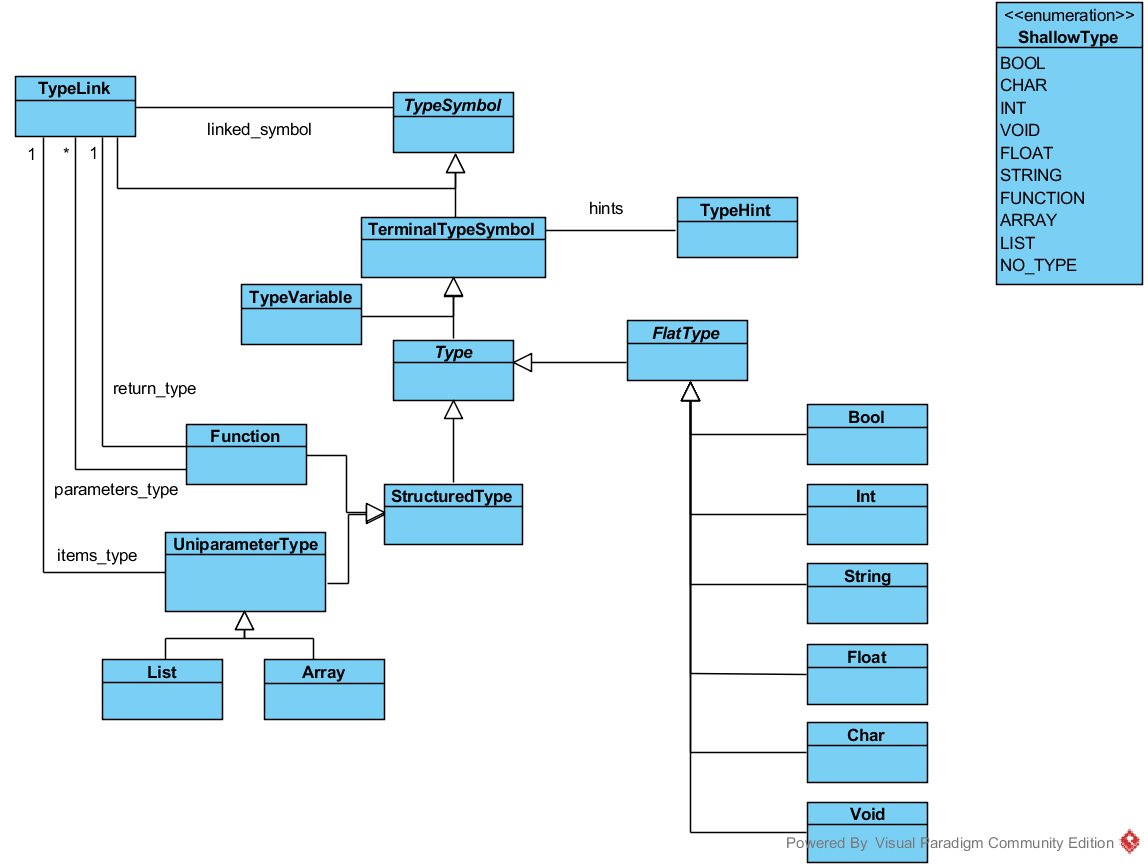
\includegraphics[scale=0.75]{type_symbols.png}
	\caption{Type symbols class diagram}
	\label{fig:}
\end{figure}

\subparagraph{Type symbol table} The type symbol table inherits from an instantiation of the C++ standard hashtable template class, \texttt{std::unordered\_map<std::string,TypeLink>}, and encapsulates the following operations :
\begin{itemize}
	\item unification between two variables
	\item unification between a variable and a flat type
	\item update of the hints of a type variable
	\item creation of new variables
	\item construction of type symbol objects for variables, functions, arrays and lists
	\item construction of a type object for the code generation phase
	\item generation of unique type variable names 
\end{itemize} 
The table stores two kind of variables : the ones bounded to the program's identifiers (so-called \textit{bounded} type variables) and the ones that are not (so-called \textit{pure} type variables). As every variable has to be uniquely identified, the generation of variable names have to be done carefully :
\begin{itemize}
	\item pure variable names are numbers generated with a counter and is therefore collision free as long as the counter does not overflow
	\item as a in a valid program, two identifiers of having the same name cannot be declared in the same scope, a unique name for bounded variables can be constructed from these two elements. An additional character, '@' is added between the identifier name and the scope id for the sake of readability mostly. The name of a bounded variable is therefore generated as follows :
	\begin{center}
		\texttt{identifier}@\texttt{scope\_id}
	\end{center}
\end{itemize}
\subparagraph{Syntax-directed type inference} The type inference is implemented with another visitor in \texttt{TypeInferenceVisitor.cpp}. Each node corresponds to a language construct of which the type semantic must be translated in the type symbol table. Moreover, a node can receive from its parent and pass to his children a set of variable (for instance, if an expression is expected to return a value of a given type, the corresponding type variable could be passed from the parent to the expression node). Therefore, designing the type inference for a node results in answering five questions :
\begin{enumerate}
	\item \textbf{Inheritance} : which type variables are inherited from the parent node?
	\item \textbf{Table insertion} : which variables must be created in the type symbol table and with which terminal type symbols have they to be associated?
	\item \textbf{Unification} : which pairs of variables have to be unified ? Does a variable have to be unified with a flat type?
	\item \textbf{Hinting} : has the hints of a variable to be updated ? 
	\item \textbf{Transmission} : which variables must be given to the children nodes?
\end{enumerate} 
As these elements must be defined for every node, the complete list is not detailed here. Nevertheless, three examples are given : the \textit{+} operator, the \textit{if} statement and the function declaration. 
\begin{itemize}
	\item \textbf{Operator +} : this node has two children, the two operands 
	\begin{itemize}
		\item \textit{Inheritance} : $\alpha$ is the type that should be returned by the operation
		\item \textit{Table insertion} : no type variable insertion 
		\item \textit{Unification} : no unification 
		\item \textit{Hinting} : as '\texttt{+}' can only take integer or float operands, we have : $\mathcal{H}_\alpha = \mathcal{H}_\alpha \cap \{\texttt{int}, \texttt{float}\}$
		\item \textit{Transmission} : as the type returned by the addition is the same as the type of the operands $\alpha$ is passed the both of them
	\end{itemize}
	\item \textbf{Statement \textit{if}} : this node has two children, the condition expression and the scope
	\begin{itemize}
		\item \textit{Inheritance} : $\alpha$ is the type that should be returned by a \texttt{nori} statement in the \textit{if} scope
		\item \textit{Table insertion} : $\beta$ is the type returned by the condition expression
		\item \textit{Unification} : as the condition expression must return a boolean value, the following unification must be performed : $unify(\beta, \texttt{bool})$
		\item \textit{Hinting} : no hinting
		\item \textit{Transmission} : $\beta$ is passed to the condition expression node and $\alpha$ to the scope node
	\end{itemize}
	\item \textbf{Function declaration} : \texttt{maki func\_name p$_1$ ... p$_n$ : scope ;;} (for instance defined in the scope 1 and its scope having id 2)
	\begin{itemize}
		\item \textit{Inheritance} : no inheritance
		\item \textit{Table insertion} : \textit{func\_name@1} is the type of the function, \textit{p$_i$@2} is the type of the $i^{th}$ parameter and $\alpha$ is the return type
		\item \textit{Unification} : the function name must be unified with the function type : 
		\[ unify(\textit{func\_name@1}, \textit{p}_1\textit{@2} \hdots \textit{p}_n\textit{@2} \rightarrow \gamma) \]
		\item \textit{Hinting} : each hinted parameter should be hinted. If the hint is a flat type, an unification can be performed instead
		\item \textit{Transmission} : $\gamma$ to the scope node
	\end{itemize}
\end{itemize}
The \textit{almost} complete list of the nodes and their inference actions is given in the \texttt{Inference.pdf} document in the submitted archive.

\section{Flaws and possible improvements}\subsection{Code generation}
\subsubsection{Code generation}
\subsubsection{Code construction}
\section{Runtime}
\subsection{Garbage collector}
\label{ssec:garabage_collector}
\appendix
\section{Sources}
\begin{enumerate}
	\item \textbf{Type inference} :
	\begin{enumerate}
		\item\label{enum:inference_unification} Paul N. Hilfinger, "\textit{Lecture \#22: Type Inference and Unification}", \texttt{https://goo.gl/RR8Eme}, UC Berekeley, course \textit{CS164} : Programming Languages and Compilers.
	\end{enumerate}
\end{enumerate}
\section{Diagrams}
\end{document}